% Copyright (C) 2013 Thomas L. Kula
% All Rights Reserved
%
% See the file LICENSE for license terms.
\documentclass[12pt]{article}
\usepackage{graphicx}
\usepackage{rotating}
\usepackage{fix-cm}
\usepackage{multirow}
\setlength{\paperwidth}{5.5in}
\setlength{\paperheight}{8.5in}
\setlength{\textheight}{7.45in}
\setlength{\topmargin}{-1.0in}
\setlength{\oddsidemargin}{-0.5in}
\setlength{\evensidemargin}{-0.5in}
\setlength{\textwidth}{4.0in}
\setlength{\parindent}{0in}
\setlength{\parskip}{3mm}
\usepackage[print]{booklet} \nofiles
\source{\magstep0}{5.5in}{8.5in}
\target{\magstep0}{11in}{8.5in}
\setpdftargetpages
\pagestyle{empty}
\begin{document}


\begin{center}
{\fontsize{36}{48}\selectfont \textsc{Haiku a Day }}
\end{center}

\vspace*{3.5cm}

{\fontsize{20}{40}\selectfont 

A breath of fresh air

Like salad after junk food

The season turns warm

}

\vspace*{5.0cm}
\begin{center}
{\large{Issue 93: March 2013}} \\[5mm]
{\fontsize{8}{8}\selectfont  \textsc{ St. Joshua Norton Press }} \\[1mm]
{\fontsize{6}{6}\selectfont Mathom House by the Cloisters \textbar The People's Republic of Ames }
\end{center}


\newpage

The windows are open, the trees are in bloom, everything is right with 
life right now.

--- Thomas

http://kula.tproa.net/had/ \\
kula@tproa.net

Download this and previous HADs at the website, so you can
print out your own (DIY, yeah!) or if you want me to send
you one, send me your address, and maybe a stamp if you
are feeling nice. Or send me something you've made ---
trades always appreciated, postcards are nice too.

\vfill

1 March 2013

Shortest to longest \\
The dreary March rain drips on \\
Will Spring ever come? 

2 March 2013

Tiny, dark and deep \\
An inglorious end waits \\
Down the garbage chute

3 March 2013

When will this fad end? \\
Adults, parading around \\
On two wheeled scooters

\newpage

4 March 2013

While doing dishes \\
I'm thinking about bubbles \\
As my mind turns off

5 March 2013

Lift up your troubles \\
Showing them the light of day \\
Sunshine's the best cure

6 March 2013

If you wear Google \\
Glasses when you're at the bar \\
You are a douchebag

7 March 2013

Errant eyebrow hair \\
Why are you freakishly long \\
Keep pulling you out

8 March 2013

A paper graveyard \\
The bottom of my pocket \\
Numerous recipts

9 March 2013

Dusk coming later \\
The days are feeling warmer \\
Spring is creeping in

10 March 2013

Ladder in the sky \\
Hanging from a hook; you drop \\
When stuff's on fire

\newpage

11 March 2013

There's a remedy \\
It involves taking a nap \\
Universal cure

12 March 2013

Too much, horrible \\
Not enough, bland and tasteless \\
Add just enough salt

13 March 2013

High upon a ridge \\
A tall tower sits, blinking \\
Keep airplanes away

14 March 2013

Bring forth onto me \\
A vast glorious breakfast \\
Need cholesterol

15 March 2013

Waiting for the queue \\
Backed-up jobs not processing \\
Go forward, minions

16 March 2013

With a faint puff, dark \\
The lightbulb gives up the ghost \\
Leaves just a dark spot

17 March 2013

The lack of coffee \\
Manifests itself: headache \\
Dull pain of a day

\newpage

18 March 2013

Dreaming of nuggets \\
Peanuts and chocolate dance \\
There is caramel

19 March 2013

Underneith the bed \\
The dust of a thousand days \\
Skitters in the breeze

20 March 2013

Do I fear scurvy? \\
A sudden craving: grapefruit \\
Eating three of them

21 March 2013

Tarrytown at night \\
The wind blowing, train horn sounds \\
Metro North back home

22 March 2013

A quiet corner \\
An 80s bachelor pad \\
Rocks sitting, dusty

23 March 2013

I am an old man \\
Concerts starting at midnight \\
Don't work well for me

24 March 2013

A song, in a loop \\
Stuck firm in a fuzzy head \\
Is how I woke up

\newpage

25 March 2013

Say bobbin, bobbin \\
The word, petulant, explodes \\
A curious bit

26 March 2013

Dirty rock and roll \\
Cider in hand, a dim room \\
Makes for a good night

27 March 2013

Cruft accumulates \\
Duct tape layers on layers \\
Time to rip it off

28 March 2013

On a ball in space \\
Floating along the cosmos \\
People fill the street

29 March 2013

Luminous sasquatch \\
Lead taco press on a shelf \\
Jibber jabber hey

30 March 2013

The late afternoon \\
Streams through the window, blinds \\
Why work? Take a walk.

31 March 2013

Simple is sometimes \\
The best way to do something \\
Don't get fancy now

\newpage

\begin{center}
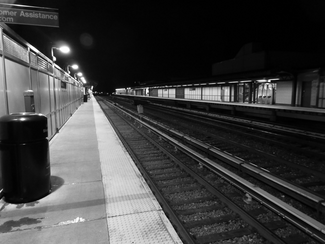
\includegraphics[width=325pt]{subway.png}
Avenue J, the BMT Brighton Line \\
9 March 2013 \\
{\tt kula.tproa.net/photos/2013/20130309-brooklyn}
\end{center}

\newpage

\thispagestyle{empty}
\vspace*{12cm}
\begin{sideways}
\Large{St. Joshua Norton Press}
\end{sideways}
\begin{sideways}
\Large{PO Box 250138}
\end{sideways}
\begin{sideways}
\Large{New York NY 10025}
\end{sideways}


\end{document}


